\section{Results}
\label{sec:results}

\subsection{Background estimate from the ABCD method}
\label{sec:abcdres}

The data yields in the 
four regions are summarized in Tables~\ref{tab:datayield1}-Table~\ref{tab:datayield3}
for the 3 signal regions. The ABCD background prediction $N_A \times N_C / N_B$ is scaled
by the correction factors determined in Sec.~\ref{sec:datadriven}, as summarized in Table~\ref{tab:cor}.

\newpage

\begin{figure}[tbh]
\begin{center}
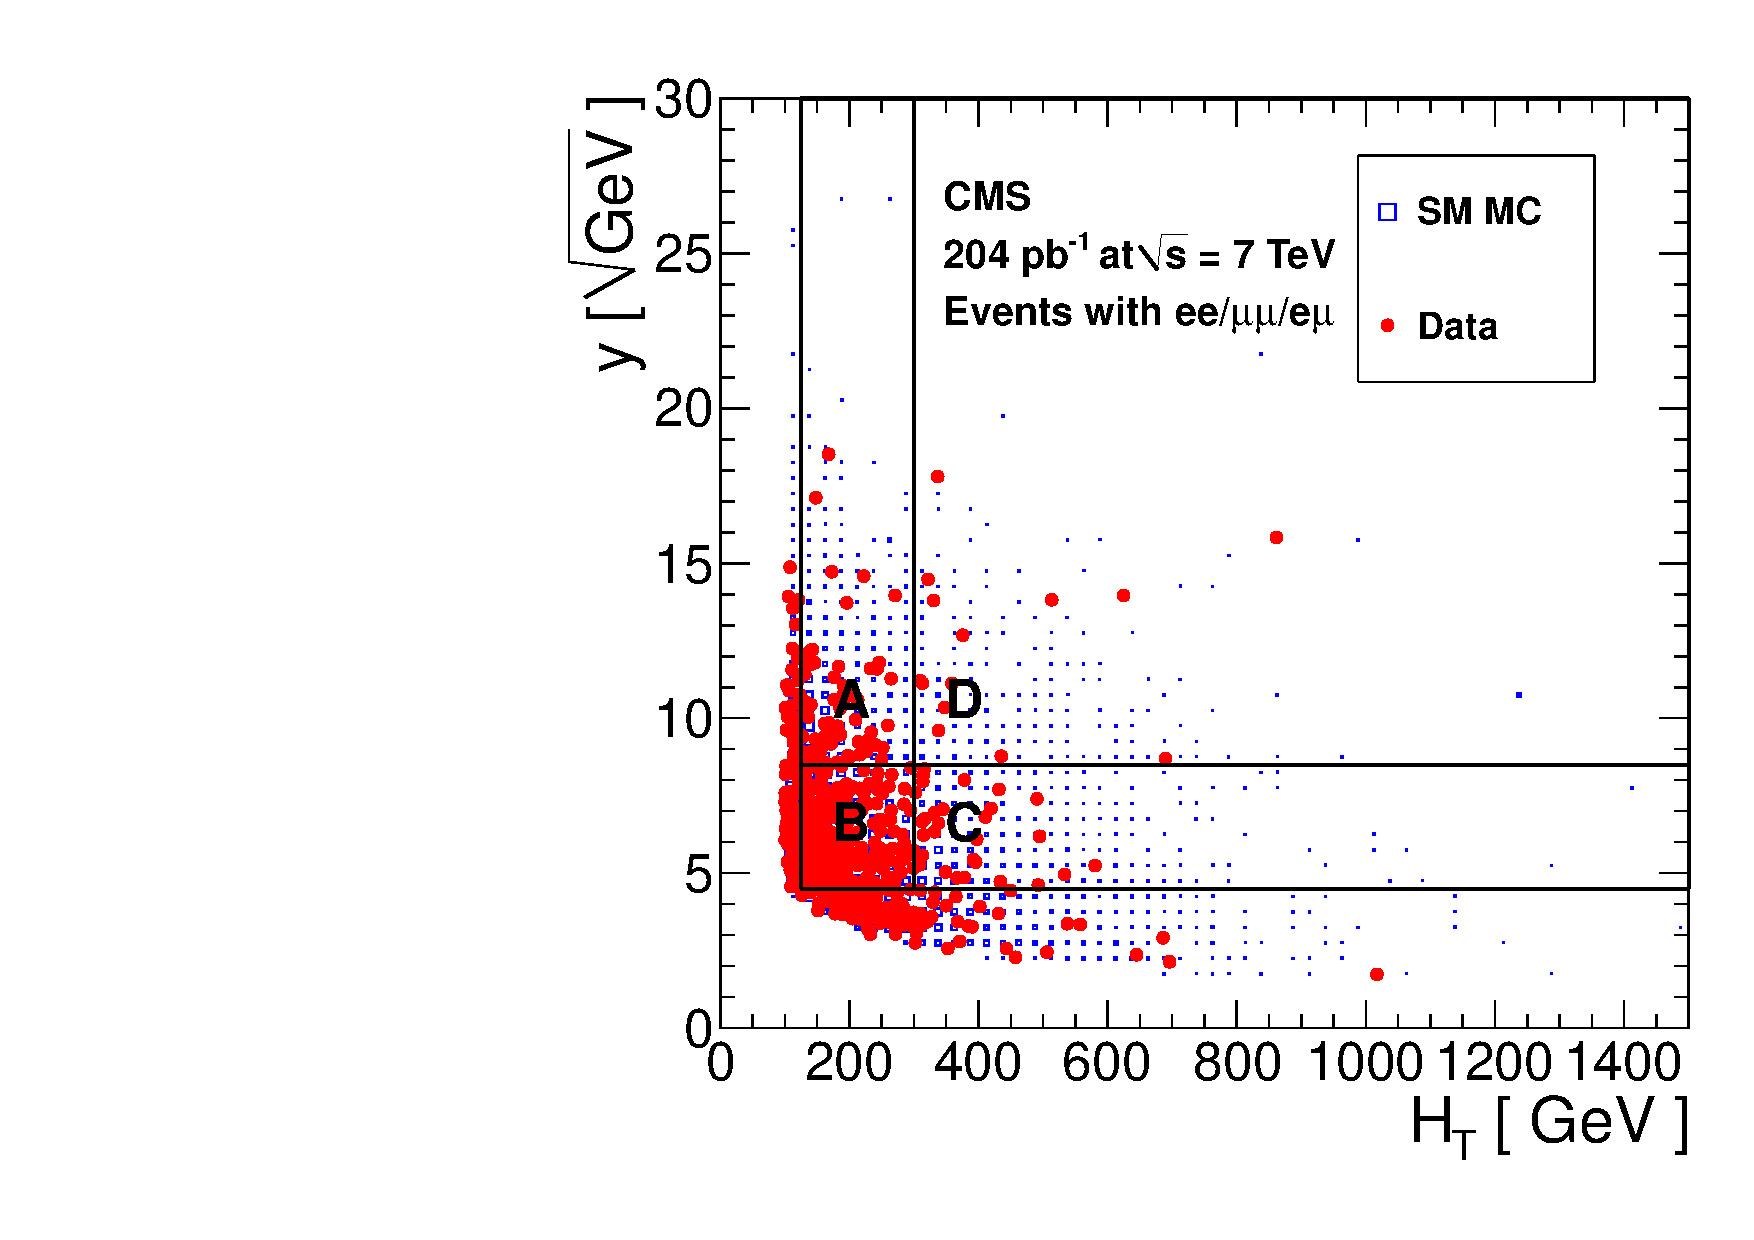
\includegraphics[width=0.6\linewidth]{plots/abcd_204pb_2010.pdf}
\caption{\label{fig:abcdData1}\protect Distributions of $y$ 
vs. \Ht\ for SM Monte Carlo and data. The 2010 signal region boundaries are overlayed.}
\end{center}
\end{figure}

\begin{table}[hbt]
\begin{center}
\caption{\label{tab:datayield1} 
Data yields in the four
regions of Figure~\ref{fig:abcdData1} for the 2010 signal region, 
as well as the predicted yield in region D given
by A $\times$ C / B.  The quoted uncertainty
on the prediction in data is statistical only, assuming Gaussian errors.
We also show the SM Monte Carlo expectations with statistical errors only.
}
\begin{tabular}{l||c|c|c|c||c}
\hline
           sample  &                A  &                B  &                C  &                D  &   A $\times$ B / C  \\
\hline
           \ttbar  & 48.8  $\pm$  1.4  &184.1  $\pm$  2.7  & 31.9  $\pm$  1.1  &  7.3  $\pm$  0.5  &  8.5  $\pm$  0.4    \\
               DY  &  0.5  $\pm$  0.4  &  8.2  $\pm$  1.5  &  0.7  $\pm$  0.5  &  1.0  $\pm$  0.6  &  0.0  $\pm$  0.0    \\
              \WW  &  0.6  $\pm$  0.1  &  1.6  $\pm$  0.1  &  0.1  $\pm$  0.0  &  0.2  $\pm$  0.0  &  0.1  $\pm$  0.0    \\
              \WZ  &  0.1  $\pm$  0.0  &  0.3  $\pm$  0.0  &  0.0  $\pm$  0.0  &  0.0  $\pm$  0.0  &  0.0  $\pm$  0.0    \\
              \ZZ  &  0.0  $\pm$  0.0  &  0.1  $\pm$  0.0  &  0.0  $\pm$  0.0  &  0.0  $\pm$  0.0  &  0.0  $\pm$  0.0    \\
       single top  &  1.9  $\pm$  0.1  &  5.6  $\pm$  0.2  &  0.2  $\pm$  0.0  &  0.1  $\pm$  0.0  &  0.1  $\pm$  0.0    \\
           \wjets  &  0.6  $\pm$  0.6  &  1.2  $\pm$  0.6  &  0.0  $\pm$  0.0  &  0.0  $\pm$  0.0  &  0.0  $\pm$  0.0    \\
\hline
      Total SM MC  & 52.6  $\pm$  1.6  &201.2  $\pm$  3.2  & 33.1  $\pm$  1.2  &  8.6  $\pm$  0.8  &  8.6  $\pm$  0.4    \\
\hline
             data  &               72  &              238  &               29  &               14  &  8.8  $\pm$  2.0    \\
\hline
\end{tabular}
\end{center}
\end{table}

\newpage

\begin{figure}[tbh]
\begin{center}
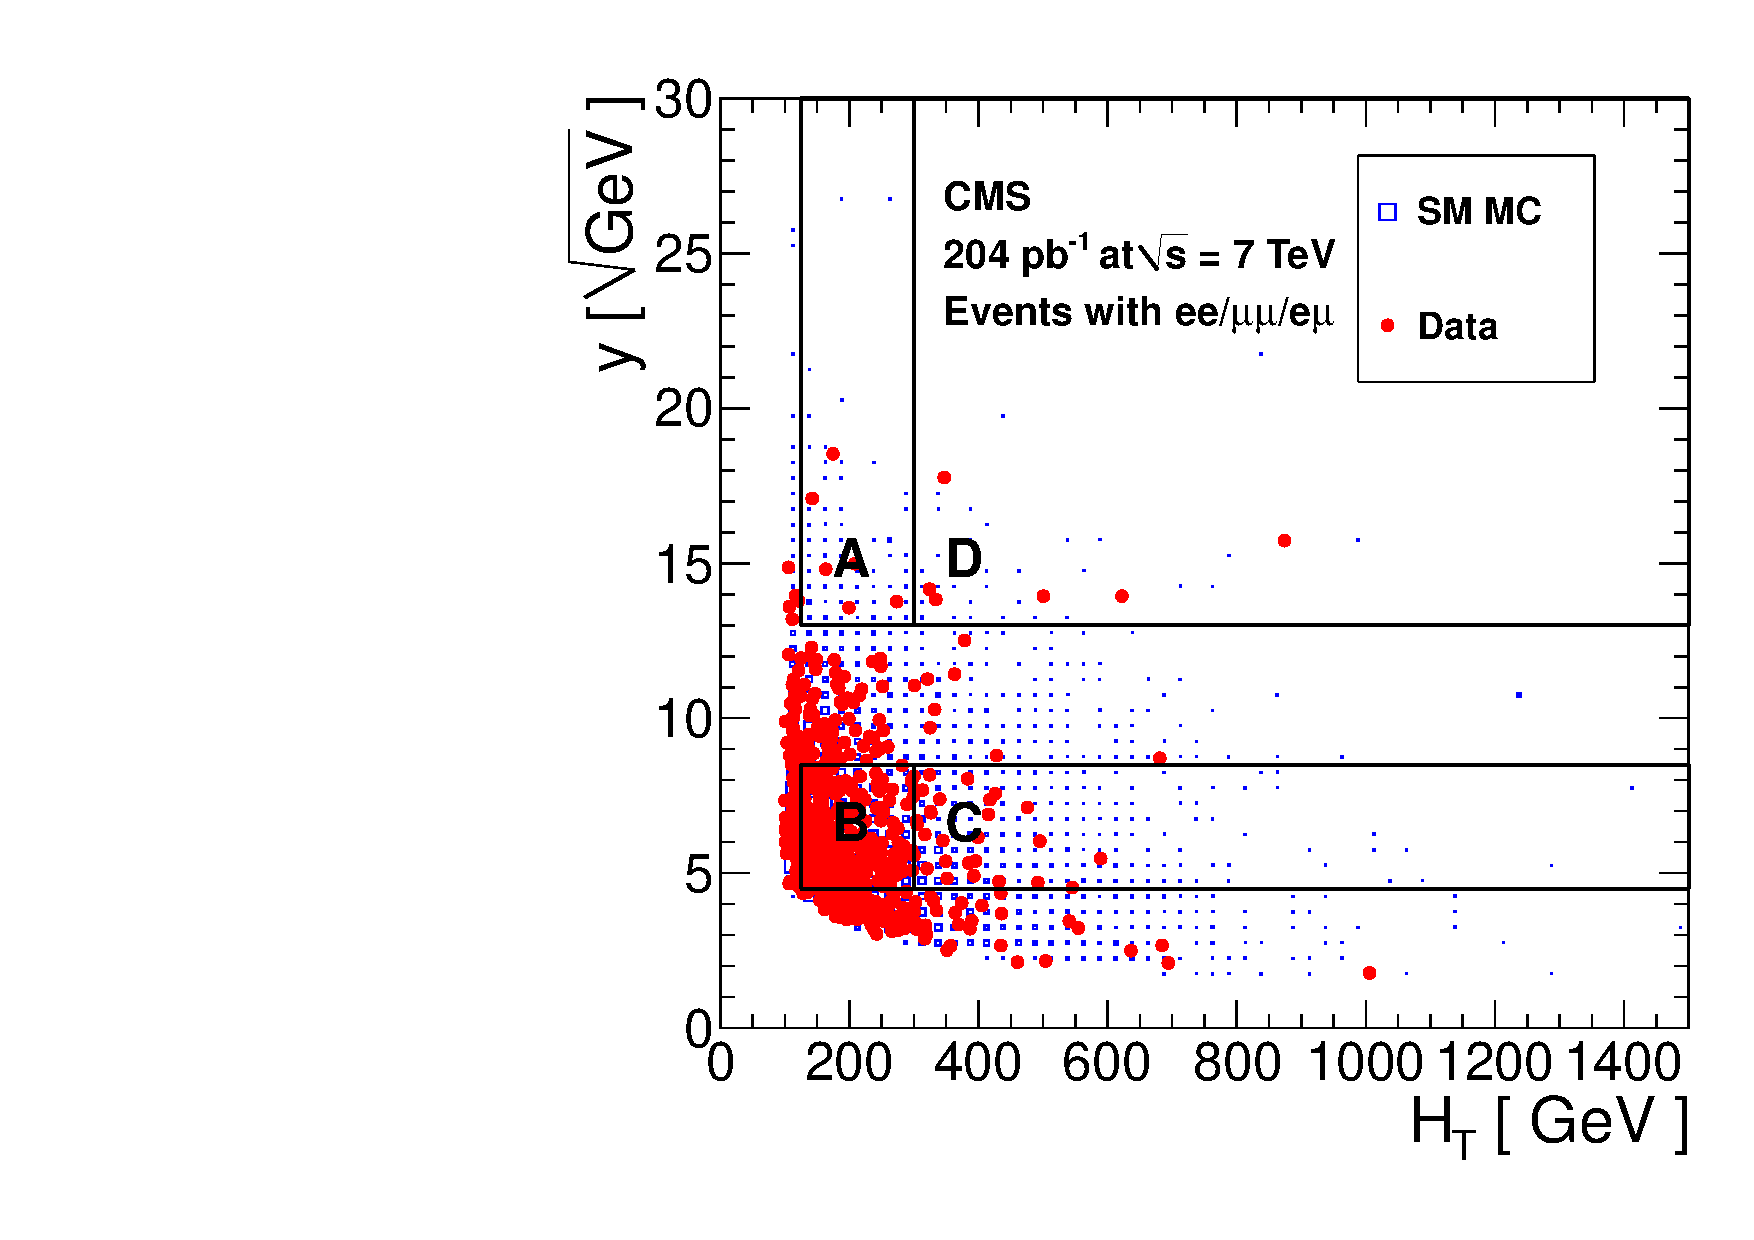
\includegraphics[width=0.6\linewidth]{plots/abcd_204pb_highy.pdf}
\caption{\label{fig:abcdData2}\protect Distributions of $y$ 
vs. \Ht\ for SM Monte Carlo and data. The high $y$ signal region boundaries are overlayed.}
\end{center}
\end{figure}


\begin{table}[hbt]
\begin{center}
\caption{\label{tab:datayield2} 
Data yields in the four
regions of Figure~\ref{fig:abcdData2} for the high $y$ signal region, 
as well as the predicted yield in region D given
by A $\times$ C / B.  The quoted uncertainty
on the prediction in data is statistical only, assuming Gaussian errors.
We also show the SM Monte Carlo expectations with statistical uncertainties.
}
\begin{tabular}{l||c|c|c|c||c}
\hline
           sample  &                A  &                B  &                C  &                D  &   A $\times$ B / C   \\
\hline
           \ttbar  &  3.6  $\pm$  0.4  &184.1  $\pm$  2.7  & 31.9  $\pm$  1.1  &  1.2  $\pm$  0.2  &  0.6  $\pm$  0.1  \\
               DY  &  0.3  $\pm$  0.3  &  8.2  $\pm$  1.5  &  0.7  $\pm$  0.5  &  0.0  $\pm$  0.0  &  0.0  $\pm$  0.0  \\
              \WW  &  0.1  $\pm$  0.0  &  1.6  $\pm$  0.1  &  0.1  $\pm$  0.0  &  0.1  $\pm$  0.0  &  0.0  $\pm$  0.0  \\
              \WZ  &  0.0  $\pm$  0.0  &  0.3  $\pm$  0.0  &  0.0  $\pm$  0.0  &  0.0  $\pm$  0.0  &  0.0  $\pm$  0.0  \\
              \ZZ  &  0.0  $\pm$  0.0  &  0.1  $\pm$  0.0  &  0.0  $\pm$  0.0  &  0.0  $\pm$  0.0  &  0.0  $\pm$  0.0  \\
       single top  &  0.2  $\pm$  0.0  &  5.6  $\pm$  0.2  &  0.2  $\pm$  0.0  &  0.0  $\pm$  0.0  &  0.0  $\pm$  0.0  \\
           \wjets  &  0.0  $\pm$  0.0  &  1.2  $\pm$  0.6  &  0.0  $\pm$  0.0  &  0.0  $\pm$  0.0  &  0.0  $\pm$  0.0  \\
\hline
      Total SM MC  &  4.1  $\pm$  0.5  &201.2  $\pm$  3.2  & 33.1  $\pm$  1.2  &  1.3  $\pm$  0.2  &  0.7  $\pm$  0.1  \\
\hline
             data  &                6  &              238  &               29  &                6  &  0.7  $\pm$  0.3  \\
\hline
\end{tabular}
\end{center}
\end{table}

\newpage

\begin{figure}[tbh]
\begin{center}
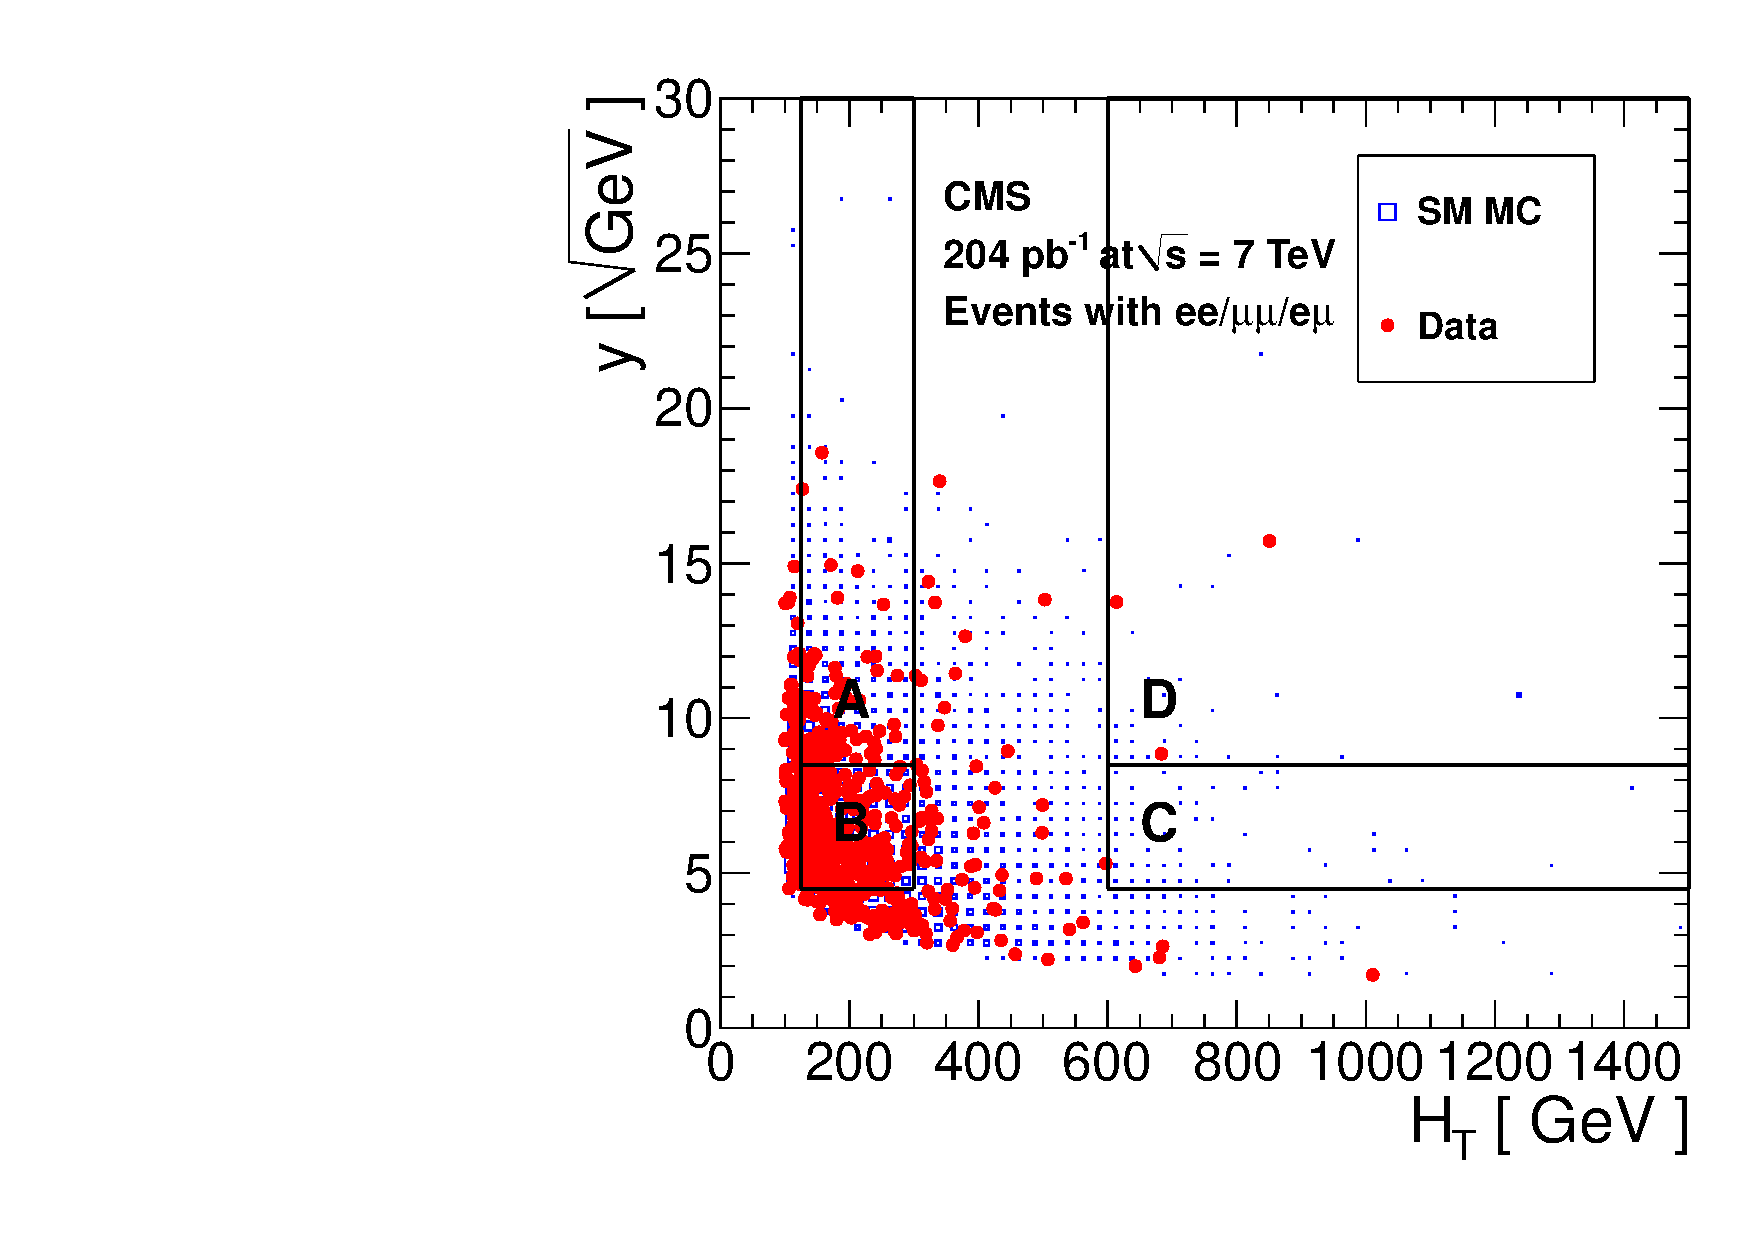
\includegraphics[width=0.6\linewidth]{plots/abcd_204pb_highht.pdf}
\caption{\label{fig:abcdData3}\protect Distributions of $y$ 
vs. \Ht\ for SM Monte Carlo and data. The high \Ht\ signal region boundaries are overlayed.}
\end{center}
\end{figure}

\begin{table}[hbt]
\begin{center}
\caption{\label{tab:datayield3} 
Data yields in the four
regions of Figure~\ref{fig:abcdData3} for the high \Ht\ signal region, 
as well as the predicted yield in region D given
by A $\times$ C / B.  The quoted uncertainty
on the prediction in data is statistical only, assuming Gaussian errors.
Since the yield in region C is 0, we assess as the uncertainty the prediction
corresponding to 1 observed event in 1.
We also show the SM Monte Carlo expectations with statistical uncertainties.
}
\begin{tabular}{l||c|c|c|c||c}
\hline
           sample  &                A  &                B  &                C  &                D  &   A $\times$ B / C  \\
\hline
            ttall  & 48.8  $\pm$  1.4  &184.1  $\pm$  2.7  &  2.2  $\pm$  0.3  &  0.7  $\pm$  0.2  &  0.6  $\pm$  0.1   \\
               DY  &  0.5  $\pm$  0.4  &  8.2  $\pm$  1.5  &  0.0  $\pm$  0.0  &  0.4  $\pm$  0.4  &  0.0  $\pm$  0.0   \\
               WW  &  0.6  $\pm$  0.1  &  1.6  $\pm$  0.1  &  0.0  $\pm$  0.0  &  0.0  $\pm$  0.0  &  0.0  $\pm$  0.0   \\
               WZ  &  0.1  $\pm$  0.0  &  0.3  $\pm$  0.0  &  0.0  $\pm$  0.0  &  0.0  $\pm$  0.0  &  0.0  $\pm$  0.0   \\
               ZZ  &  0.0  $\pm$  0.0  &  0.1  $\pm$  0.0  &  0.0  $\pm$  0.0  &  0.0  $\pm$  0.0  &  0.0  $\pm$  0.0   \\
                t  &  1.9  $\pm$  0.1  &  5.6  $\pm$  0.2  &  0.0  $\pm$  0.0  &  0.0  $\pm$  0.0  &  0.0  $\pm$  0.0   \\
            wjets  &  0.6  $\pm$  0.6  &  1.2  $\pm$  0.6  &  0.0  $\pm$  0.0  &  0.0  $\pm$  0.0  &  0.0  $\pm$  0.0   \\
\hline
      Total SM MC  & 52.6  $\pm$  1.6  &201.2  $\pm$  3.2  &  2.2  $\pm$  0.3  &  1.2  $\pm$  0.5  &  0.6  $\pm$  0.1   \\
\hline
             data  &               72  &              238  &                0  &                3  &  0.0  $\pm$  0.3   \\
\hline
\end{tabular}
\end{center}
\end{table}

\newpage

%\clearpage

\begin{table}[hbt]
\begin{center}
\caption{\label{tab:victory} 
Summary of results of the ABCD method, applied to the 3 signal regions.
}
\begin{tabular}{lccccc}
\hline
Signal Region           &  $N_A \times N_C / N_B$   &  correction factor         &  prediction    \\ 
\hline
2010 signal region      &          $8.8 \pm 2.0$    & $1.0 \pm 0.2$             & 8.8 $\pm$ 2.0 (stat) $\pm$ 1.8 (syst)  \\
high $y$ signal region  &          $0.7 \pm 0.3$    & $1.3 \pm 0.2$             & 0.9 $\pm$ 0.4 (stat) $\pm$ 0.2 (syst)  \\
high \Ht\ signal region &          $0.0 \pm 0.3$    & $1.2 \pm 0.2$             & 0.0 $\pm$ 0.4 (stat) $\pm$ 0.1 (syst)  \\
\hline
\end{tabular}
\end{center}
\end{table}

\subsection{Background estimate from the $P_T(\ell\ell)$ method}
\label{sec:victoryres}

\begin{table}[hbt]
\begin{center}
\caption{\label{tab:victory} 
Summary of results of the dilepton $p_{T}$ template method.
The number of events in the given signal region with the $y$ requirement replaced by a \ptht\
requirement is $N(D')$, the estimated DY contribution from the $R_{out/in}$ technique is $N(DY)$,
the \met\ acceptance scaling factor is $K$, the residual correction factor is $K_C$, and
the the prediction from the \ptll\ method is $N_P$. The quoted statistical uncertainty is due to
that of $N(D')$, the quoted systematic uncertainty includes that of $N(DY)$ and $K_C$.
{\bf K and KC taken from MC, do we want to take K and/or KC from data? }
{\bf Need to add jet/met uncertainty here}
%{\color{red} \bf CURRENTLY USING 30\% UNCERTAINTY ON K_C IN 2010 REGION, WHICH IS WHAT WE HAD LAST YEAR (NEED TO REPEAT JET/MET UNCERTAINTIES?).}
%{\color{red} \bf FOR HIGH Y/HIGH HT REGION, TAKING SYST UNCERTAINTY ON KC FROM MC STATS, WHICH IS PROBABLY DOMINANT}
}
\begin{tabular}{lccccc}
\hline
Signal Region           &  $N(D')$   &   $N(DY)$         &  $K$   &   $K_C$          & $N_P$  \\ 
\hline
2010 signal region      &      3     &   $0.4 \pm 0.3$   &  1.5   &   $1.4 \pm 0.2$  & 5.5 $\pm$ 3.6 (stat) $\pm$ 1.0 (syst) \\
high $y$ signal region  &      2     &   $0.1 \pm 0.1$   &  1.5   &   $1.7 \pm 0.3$  & 4.8 $\pm$ 3.6 (stat) $\pm$ 0.9 (syst) \\
high \Ht\ signal region &      0     &   $0.0 \pm 0.1$   &  1.3   &   $1.3 \pm 0.2$  & 0.0 $\pm$ 1.7 (stat) $\pm$ 0.3 (syst) \\
\hline
\end{tabular}
\end{center}
\end{table}

For each signal region D, we count the number of events falling in the region D', which is defined
using the same requirements as D but switching the $y$ requirement to a $\ptll/\sqrt{H_T}$ requirement.
We subtract off the expected DY contribution using the data-driven $R_{out/in}$ technique, using $R_{out/in} = 0.13 \pm 0.07$.
{\color{red} \bf add plot justifying this value}. We then scale this yield by 2 corrections factors:
$K$, the \met\ acceptance correction factor, and $K_C$, the correction factor determined in Sec.~\ref{sec:datadriven}.
Our final prediction $N_P$ is given by the following, as summarized in Table~\ref{tab:victory}:

\begin{center}
$ N_P = (N(D')-N(DY)) \times K \times K_C$.
\end{center}

{\color{red} \bf I will add here the results of victory method applied to the \Ht\ sideband region as a validation of the method }

% \clearpage
\subsection{Summary of results}


\begin{table}[hbt]
\begin{center}
\caption{\label{tab:victory} 
Summary of the observed and predicted yields in the 3 signal regions.
{\color{red} \bf currently just taking ee+mm-em for OF subtraction, need to update with efficiency/trig correction}.
}
\begin{tabular}{lccccc}
\hline
Signal Region                          &  2010 signal region   &   high $y$ signal region  &  high \Ht\ signal region     \\ 
\hline
Observed yield                         &         14            &                        6  &                        3     \\
MC prediction           
ABCD prediction                        &
\ptll\ prediction                      &
OF subtraction ($ee + \mu\mu - e\mu$)  &
\end{tabular}
\end{center}
\end{table}

In summary, we observe a slight excess of events with respect to MC and data-driven predictions in our loose 2010 signal region.
The excess with respect to MC and ABCD predictions is enhanced after tightening the $y$ requirement, but the observed
yield shows no significant excess with respect to the \ptll\ method prediction. There is also a slight excess of events
with respect to MC and data-driven predictions for the high \Ht\ signal region. 
